
%%%
% Any line that begins with a percent symbol is a comment. To compile
% this document and view the output:
%
% Run Latex
% Run Bibtex
% Then run Latex twice.
%
% This should produce the output PDF file named main.pdf
%%%

% This defines the style to use for this document.
% Do not modify.
\documentclass[letterpaper]{article}

% The following are akin to "import" statements in Python or Java -
% these import useful commands into the document for you to use.  You
% don't have to modify any of these lines. The AAAI package formats
% this document in the style of submissions to the American
% Association for Artificial Intelligence conference, one of the top
% AI conferences in the world. You will find that many academic
% publications in AI use this format.
\usepackage{aaai} 
\usepackage{times} 
\usepackage{helvet} 
\usepackage{courier} 
\setlength{\pdfpagewidth}{8.5in} 
\setlength{\pdfpageheight}{11in} 
\usepackage{amsmath}
\usepackage{amsthm}
\usepackage{graphicx}
\usepackage{graphics}
\usepackage{moreverb}
\usepackage{subfigure}
\usepackage{epsfig}
\usepackage{txfonts}
\usepackage{palatino}
\usepackage{algpseudocode}
\usepackage{multirow, multicol}
\usepackage{url}
\usepackage{tablefootnote}
\usepackage{color}
\usepackage{ upgreek }


\setcounter{secnumdepth}{1}
\nocopyright

% Fill in your paper title, names and emails below
% The "\\" is used to break lines. The \url command
% is useful for typesetting URLs and email addresses (it uses the
% Courier font).
\title{Depth Image Region Segmentation}
 \author{Jackson Spell \and Micah Brown\\
 \url{{jaspell,msbrown}@davidson.edu}\\
 Davidson College\\
 Davidson, NC 28035\\
 U.S.A.}

% This is the "true" start of the document. All the text in your
% write-up should be placed within the \begin{document} and
% \end{document} decorators.
\begin{document}

\maketitle % formats the title nicely, do not modify

% While at this point you could just begin your write-up, often, it's
% useful to write each section of your write-up in a separate tex
% file (not unlike the modular decomposition you do for code you
% write). These \input commands insert the contents of the
% specified tex files in the order specified. Every write-up you
% submit must contain the following sections, in the shown order. Open
% each of the indicated tex files to understand what goes in each
% section, as well as for more TeX tips.

% Place the contents of your abstract between the
% \begin{abstract} and \end{abstract} decorators.

\begin{abstract}

Segmentation algorithms separate an image into unique regions
determined by characteristics of the pixels within those regions.
Image segmentation has applications in Artificial Intelligence,
including computer vision, 3D modeling, and robotics.  We use two
different algorithms to segment a depth image, which encodes distance information into rather than conventional
RGB values.  Whereas color images are commonly segmented into regions
of similar color or luminosity, we segment the depth image into
cohesive surfaces using gradient difference and Laplacian edge detection. When combined together, these two
methods offer a chance to reconstruct three dimensional objects from
depth data.

\end{abstract}



% The \section{} command formats and sets the title of this
% section. We'll deal with labels later.
\section{Introduction}
\label{sec:intro}
Image processing is a vital component of computer vision and
artificial intelligence. Within image processing, image segmentation
continues to be a focus of research as machines are expected to be
able to have similar visual abilities as humans. Image segmentation
divides an image into regions of similar characteristics, which
ultimately can lead to object recognition. 

Depth images contain information about the distance a point in space
is to the camera eye. Whereas traditional RGB images contain a matrix
of pixels, each containing a red, green, and blue value, a depth image
only contains a matrix of depth values. Depth images can be visually
rendered as black and white images, where a point of maximum distance
is represented as white and a point of minimum distance is represented
as black. Accurate depth images were hard to construct until the
invention of modern technologies. Notably, the Microsoft Xbox Kinect
sensor has the ability to simultaneously record depth images and color
images, providing researchers easy access to rich depth data.\\

There are two main approaches for segmenting an image: edge-based
segmentation and region-based segmentation \cite{aima}. Edge-based
segmentation locates major discontinuities in the image, indicating
separate distinguishable objects, whereas region-based segmentation
identifies different surfaces within those objects by calculating the
normal vectors at each point. The remainder of this paper will go over
background information pertaining to the two methods of segmentation,
describe our specific experimental design, and share our results. 

% In this section, you should introduce the reader to the problem you
% are attempting to solve. For example, for the first project: describe
% the $15$-puzzle, and why it's interesting as an A.I. problem. You
% should also cite and briefly describe other related papers that have
% tackled this problem in the past --- things that came up during the
% course of your research. In the AAAI style, citations look like
% \cite{aima} (see the comments in the source file \texttt{intro.tex} to
% see how this citation was produced). Conclude by summarizing how the
% remainder of the paper is organized. \\

% Citations: As you can see above, you create a citation by using the
% \cite{} command. Inside the braces, you provide a "key" that is
% uniue to the paper/book/resource you are citing. How do you
% associate a key with a specific paper? You do so in a separate bib
% file --- for this document, the bib file is called
% project1.bib. Open that file to continue reading...

% Note that merely hitting the "return" key will not start a new line
% in LaTeX. To break a line, you need to end it with \\. To begin a 
% new paragraph, end a line with \\, leave a blank
% line, and then start the next line (like in this example).
% Overall, the aim in this section is context-setting: what is the
% big-picture surrounding the problem you are tackling here?



\section{Background}
\label{sec:background}

\subsection{Laplacian Edge Detection}
\label{subsec:laplacian}
Edge detection attempts to distinguish solid objects in an image. This
method of segmentation relies on the fact that edges of an image will
have large discontinuities in the data. In color images, two different
objects often have very different luminosities, colors, or
brightnesses; edge detection locates the areas where the pixels
experience a rapid change in those values. While pixels in RGB images
have these various characteristics, depth image pixels only have one
piece of data (the depth). Thus, edge detection in depth images
locates objects in an image by finding the areas in which the depth
data rapidly changes. 

To find this area, a Gaussian blur convolution is first applied to the
depth image. Then, the blurred image, $image_{blur}$, is subtracted
from the original image, $image_{original}$, resulting in the
``edged'' image, $image_{edged}$. Areas with similar values are
relatively unchanged after the blur, and result in low values in
$image_{edged}$. However, the areas    

\subsection{Gradient Surface Detection}
\label{subsec:gradient}
Background information on G.S.D. goes here.

% Describe any background information that the reader would need to know
% to understand your work. You do not have to explain algorithms or
% ideas that we have seen in class. Rather, use this section to describe
% techniques that you found elsewhere in the course of your research,
% that you have decided to bring to bear on the problem at hand. Don't
% go overboard here --- if what you're doing is quite detailed, it's
% often more helpful to give a sketch of the big ideas of the approaches
% that you will be using. You can then say something like ``the reader
% is referred to X for a more in-depth description of...'', and include
% a citation.\\
% Alternately, you may have designed a novel approach for the problem
% --- your own algorithm or heuristic, say. A description of these would
% also be placed in this section (use subsections to better organize the
% content in this case).

% % Note the \subsection{} command 
% \subsection{Enumerating}
% \label{subsec:enum}

% Create bulleted lists by using the \texttt{itemize} command (see source code):
% \begin{itemize}
%   \item Item 1
%   \item Item 2
%   \item Item 3
% \end{itemize}
% Create numbered lists by using the \texttt{enumerate} command (see source code):
% \begin{enumerate}
%   \item Item 1
%   \item Item 2
%     \begin{enumerate}
%     \item Sub-item 2a
%     \item Sub-item 2b
%     \end{enumerate}
%   \item Item 3
% \end{enumerate}

% \subsection{Formatting Mathematics}
% \label{subsec:math}

% Entire books have been written about typesetting mathematics in
% \LaTeX~, so this guide will barely scratch the surface of what's
% possible. But it contains enough information to get you started, with
% pointers to resources where you can learn more. First, the basics: all
% mathematical content needs to be written in ``math-mode'' --- this is
% done by enclosing the content within \$ symbols. For example, the code
% to produce $6x + 2 = 8$ is \texttt{\$6x + 2 = 8\$}. Note that this is
% only good for inline math; if you would like some stand-alone math on
% a separate line, use \emph{two} \$ symbols. For example,
% \texttt{\$\$6x + 2 = 8\$\$} produces: $$6x+2 = 8$$ Here are various
% other useful mathematical symbols and notations --- see the source
% code to see how to produce them.

% \begin{itemize}
%   \item Sub- and super-scripts: $e^{x}, a_{n}, e^{2x+1}, a_{n+2}, f^{i}_{n+1}$
%   \item Common functions: $\log{x}, \sin{x}$
%   \item Greek symbols: $\epsilon, \phi, \pi, \Pi, \Phi$ % capitalizing the first letter produces the upper case letter
%   \item Summations: $\sum_{i=0}^{i=100} i^{2}$ % looks nicer if you typeset it on its own line using $$
%   \item Products: $\prod_{i=0}^{\infty} 2^{-i}$
%   \item Fractions: $3/2$ % prefer this look for inline math
%     $$\frac{x + 5}{2 \cdot \pi}$$\\ % only looks nice when typeset on its own line
% \end{itemize}

% \noindent Other useful resources:
% \begin{itemize}
% \item Find the \LaTeX~command you're looking for by drawing what you
%   want to produce\footnote{Thanks to Dr. Kate Thompson for pointing me
%     to this resource. Also, this is how you create a footnote. Also,
%     don't overuse them --- prefer citations and use the
%     acknowledgements section when possible. I usually only use
%     footnotes when I want to link to include a pointer to a web
%     site.}:\url{http://detexify.kirelabs.org/classify.html}
% \item Ask others: \url{http://tex.stackexchange.com/}
% \item Every \LaTeX~symbol ever:\\ \url{http://tinyurl.com/6s85po}

% \end{itemize}




\section{Algorithms}
\label{sec:expts}

Our research sought to determine whether the Laplacian Edge Detection method or the Gradient Surface Detection method would produce more better segmentation on depth images. Our detailed algorithms are outlined below. In Laplacian Edge Detection, a convolution matrix was built with a $radius = 8$ and $\sigma = \frac{7}{3}$, which we found resulted in a smooth blur. We used a threshold of 4 to determined whether an edge had been located. Using a low threshold resulted in well defined edges but presented several false artifacts as an unintended side-effect.

\begin{algorithm}
\caption{Laplacian Edge Detection (Image $depth$)}\label{laplacian}
\begin{algorithmic}[1]
\State Image $segmented \gets$ \textbf{new} Image
\State Image  $blur \gets$ \textbf{new} Image
\State $blur \gets $ \Call{GaussianBlur}{Horizontal, $depth$}
\State $blur \gets $ \Call{GaussianBlur}{Vertical, $blur$}
\For{$i$ \textbf{in} $length$, $j$ \textbf{in} $height$}
\State $segmented_{i, j} \gets (original_{i, j}-blur_{i, j}$)
\If {$segmented_{i,j} > threshold$}
\State \textbf{label} $segmented_{i,j}$ Edge
\EndIf
\EndFor
\item[]
\For{Pixel $p$ \textbf{in} $segmented$}
\If {$p$ \textbf{is not} visited}
\State $region \gets$ \Call{FloodFill}{$p$} 
\For{Pixel $q$ \textbf{in} $region$}
\State \textbf{label} $q$ visited
\EndFor
\EndIf
\EndFor
\State \Return{$segmented$}
\end{algorithmic}
\end{algorithm}

Gradient Surface Detection relies on accurate calculations of the surface normals. First, the gradient is calculated in the horizontal direction by taking the difference of the two depths on either side of the pixel. This gradient, $\Delta$horizontal, represents the horizontal vector of the surface. Then the value of the angle of this vector is found by: 
\begin{equation}\label{theta}\theta = \tan^{-1}{(\frac{p_{i+1,j}-p_{i-1,j}}{2})} \end{equation}
Similarly, the vertical gradient, $\Delta$vertical, is found by:
\begin{equation}\label{phi}\theta = \tan^{-1}{(\frac{p_{i,j+1}-p_{i,j-1}}{2})} \end{equation}
Now, using \eqref{theta} and \eqref{phi}, we calculate the normal vector to both of those vectors as:
\begin{equation}\label{psi}\psi = \cos^{-1}{(\cos{\theta_1}\cos{\theta_2} + \sin{\theta_1}\sin{\theta_2}\cos{(\theta_1-\theta_2)})} \end{equation}
In particular, $\psi$ is derived from the spherical law of cosines. For this algorithm, a threshold of .6 (radians) was used to determine whether one surface normal differed greatly from another. A "maximum jump" parameter was added to solve the case of two normals being adjacent (due to perspective) in a depth image, despite them being far away from each other. For example, a depth image of an open doorway may have the walls surrounding the door at a normal pointing directly at the eye, and the normals of the wall that is through the open door pointing the same direction. These are two distinct surfaces that ideally this algorithm could detect, yet their normals are identical. By setting $max_jump =  10$, we are saying that if adjacent pixels differ by more than $10$ centimeters, they cannot be on the same surface.



\begin{algorithm}
\caption{Gradient Surface Detection (Image $depth$)}\label{gradient}
\begin{algorithmic}[1]
\For{Pixel $p$ \textbf{in} $depth$}
\State $p_{norm} \gets$ Normal($p$) 
\EndFor
\For{Pixel $p$ \textbf{in} $depth$}
\If{$p$ \textbf{not} visited}
\State \textbf{label} $p$ visited
\State $region \gets \Call{Regionify}{p, region}$
\EndIf
\EndFor
\item[]
\Procedure{Regionify}{Pixel $p$, List $region$}
\For{Pixel $q$ in Neighbors($p$)}
\If{$q$ \textbf{not} visited \textbf{and} 
\Statex[4] Angle($p_{norm}$, $q_{norm}$) $<threshold$ \textbf{and} 
\Statex[4] $|p-q|<max\_jump$}
\State Append $region$ \textbf{with} $q$
\State \textbf{label} $q$ visited
\State \Call{Regionify}{$q,region$}
\EndIf
\EndFor
\State \Return $region$
\EndProcedure
\end{algorithmic}
\end{algorithm}


\section{Results}
\label{sec:results}

Present the results of your experiments. Simply presenting the data is
insufficient! You need to analyze your results. What did you discover?
What is interesting about your results? Were the results what you
expected? Use appropriate visualizations. Prefer graphs and charts to
tables as they are easier to read (though tables are often more
compact, and can be a better choice if you're squeezed for space).
\textbf{Always} include information that conveys the uncertainty in
your measurements: mean statistics should be plotted with error bars,
or reported in tables with a $\pm$ range. The $95\%$-confidence
interval is a commonly reported statistic.

% \subsection{Embedding Pictures}
% \label{subsec:pics}

% See the source code (\texttt{results.tex}) for instructions on how to
% insert figures (like figure~\ref{fig:tex}) or plots into your
% document.

% % Note that TeX has a mind of its own when it comes to placing images
% % in documents - where a figure appears in the PDF document will often
% % be quite different from where it appears in the source code. This is
% % a feature, not a bug - it enables LaTeX to produce layouts that
% % "flow" better. It only takes a few lines to insert a figure into
% % your write-up - I recommend using PNG, JPG or PDF images
% % (incidentally, programs like Excel and Matlab will allow you to save
% % any plots or figures you generate in those formats). The \figure{}
% % command is used to create a new figure.
% \begin{figure}[htb]

%   \centering  % centers the image in the column

%   % replace the second argument below with your filename. I like to
%   % place all my figures in a sub-directory to keep things organized
%   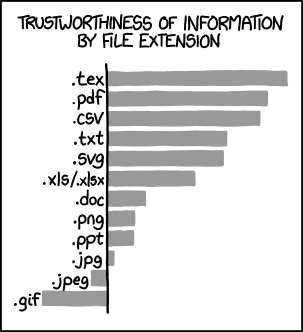
\includegraphics[width=0.47\textwidth]{figs/file_extensions.png}

%   % *Every* figure should have a descriptive caption.
%   \caption{On the trustworthiness of \LaTeX. Image courtesy of \texttt{xkcd}.}

%   % The label is a handle you create so that you can refer to this
%   % figure (using the \ref{} command) from other parts of your
%   % document. LaTeX automatically renumbers figures and updates
%   % references when you recompile, so you should do it this way rather
%   % than hard-coding in references. Notice that I've also been
%   % creating labels for the various sections in the document; I could
%   % use \ref{} command to refer to those sections using their labels
%   % too.
%   \label{fig:tex}

% \end{figure}

% \subsection{Creating Tables}
% \label{subsec:tables}

% Again, refer to \texttt{results.tex} to learn how to create simple
% tables (like table~\ref{tab:example}).
% \begin{figure}[htb]
%   \centering % centers the entire table

%   % The following line sets the parameters of the table: we'll have
%   % three columns (one per 'c'), each
%   % column will be centered (hence the 'c'; 'l' or 'r' will left or
%   % right justify the column) and the columns
%   % will have lines between them (that's the purpose of the |s between
%   % the 'c's).
%   \begin{tabular}{|c|c|c|} 
%     \hline \hline % draws two horizontal lines at the top of the table
%     Column 1 & Column 2 & Column 3 \\ % separate column contents using the &
%     \hline % line after the column headers
%     $1$ & $3.1$ & $2.7$ \\
%     $42$ & $-1$ & $1729$\\
%     \hline \hline
%   \end{tabular}

%   % As with figures, *every* table should have a descriptive caption
%   % and a label for ease of reference.
%   \caption{An example table.}
%   \label{tab:example}

% \end{figure}



\section{Conclusions}
\label{sec:concl}

We have developed two algorithms for depth image segmentation, one using the Marr-Hildreth algorithm (Laplacian Edge Detection) and one grouping pixels by normal vector (Gradient Surface Detection).  Those algorithms were tested on images of normal domestic scenes taken by an Xbox Kinect sensor, providing a realistic and varied environment.  We found that LED segmented based on jump discontinuities, locating disconnected objects, and GSD located surfaces within each object.

Because LED and GSD segment an image based on different qualities, their results provide different information.  LED finds disconnected objects, but provides no information about the shape of the object.  GSD describes the structure of each surface within the image, but cannot group surfaces to approximate a total object.  Further research in these algorithms could investigate a combination of the two, using LED to locate objects and GSD to separate them into surfaces, allowing an object to be recognized as a system of planes and facilitating automated modeling.  

We frequently found that characteristics in parts of an image -- small details, flaws in image quality, etc. -- governed the choice of parameters for the entire image, which limited the performance of both algorithms across the image as a whole.  An analysis function designed to tune parameters for sections of an image would allow the algorithms to perform effectively across the image, and would significantly increase the value of the algorithms presented.

\section{Acknowledgements} 
\label{sec:ack} 

This section is optional. But if there are people you'd like to thank for their help with the project --- a person who contributed some insight, friends who volunteered to help out with data collection, etc. --- then this is the place to thank them. Keep it short!


% This creates the references section. Open the project1.bib file to
% see how to organize your references.
\bibliography{project1}
\bibliographystyle{aaai} % sets citation and bib style, do not modify

\end{document}
